% Asset ID: AS1VectorsTikZ-001
% Source: P1-Chp11-Vectors.pdf, Vector Basics slide; Chapter_11_Vectors transcript
% Related lesson section: Key Definitions and Notation; Core Theory: Vector Basics
% Purpose: Show that a vector is a displacement with magnitude and direction, and that equal vectors can appear in different locations.
\documentclass[tikz,border=8pt]{standalone}
\usepackage{amsmath}
\usepackage{bm}
\usetikzlibrary{arrows.meta,positioning,angles,quotes}
\begin{document}

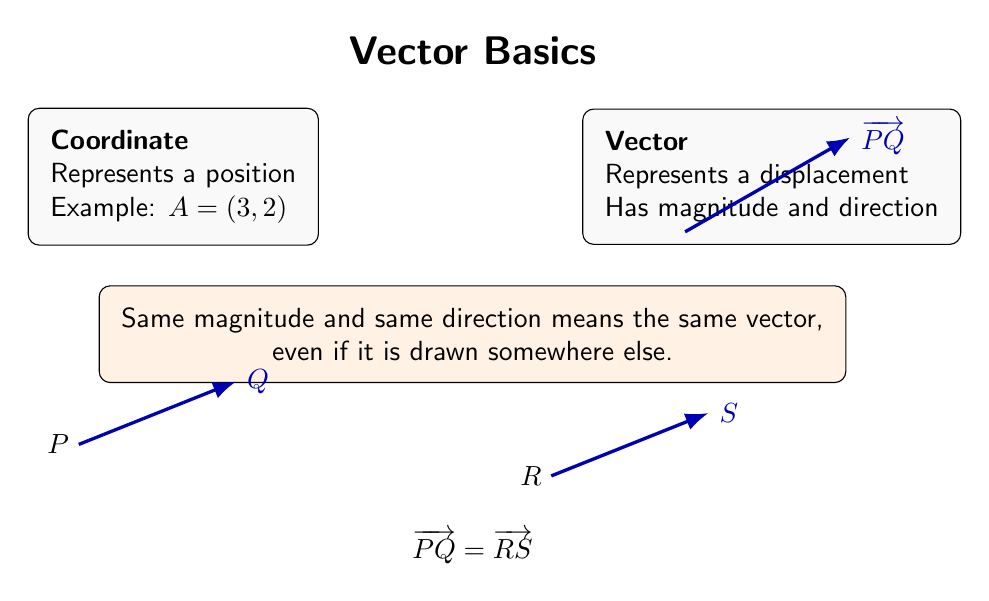
\begin{tikzpicture}[>=Latex,every node/.style={font=\sffamily},vector/.style={->,very thick,blue!70!black}]
\node[font=\sffamily\bfseries\Large] at (0,4) {Vector Basics};
\node[draw,rounded corners,fill=gray!5,align=left,inner sep=8pt] at (-3.8,2.4) {\textbf{Coordinate}\\Represents a position\\Example: $A=(3,2)$};
\node[draw,rounded corners,fill=gray!5,align=left,inner sep=8pt] at (3.8,2.4) {\textbf{Vector}\\Represents a displacement\\Has magnitude and direction};
\draw[vector] (2.7,1.7)--(4.8,2.9) node[right] {$\overrightarrow{PQ}$};
\node[draw,rounded corners,fill=orange!10,align=center,inner sep=8pt] at (0,.4) {Same magnitude and same direction means the same vector,\\even if it is drawn somewhere else.};
\draw[vector] (-5,-1)--(-3,-.2) node[right] {$Q$};\node[left] at (-5,-1) {$P$};
\draw[vector] (1,-1.4)--(3,-.6) node[right] {$S$};\node[left] at (1,-1.4) {$R$};
\node at (0,-2.3) {$\overrightarrow{PQ}=\overrightarrow{RS}$};
\end{tikzpicture}

\end{document}
